\documentclass[]{article}
\usepackage{lmodern}
\usepackage{amssymb,amsmath}
\usepackage{ifxetex,ifluatex}
\usepackage{fixltx2e} % provides \textsubscript
\ifnum 0\ifxetex 1\fi\ifluatex 1\fi=0 % if pdftex
  \usepackage[T1]{fontenc}
  \usepackage[utf8]{inputenc}
\else % if luatex or xelatex
  \ifxetex
    \usepackage{mathspec}
    \usepackage{xltxtra,xunicode}
  \else
    \usepackage{fontspec}
  \fi
  \defaultfontfeatures{Mapping=tex-text,Scale=MatchLowercase}
  \newcommand{\euro}{€}
\fi
% use upquote if available, for straight quotes in verbatim environments
\IfFileExists{upquote.sty}{\usepackage{upquote}}{}
% use microtype if available
\IfFileExists{microtype.sty}{%
\usepackage{microtype}
\UseMicrotypeSet[protrusion]{basicmath} % disable protrusion for tt fonts
}{}
\usepackage{graphicx}
\makeatletter
\def\maxwidth{\ifdim\Gin@nat@width>\linewidth\linewidth\else\Gin@nat@width\fi}
\def\maxheight{\ifdim\Gin@nat@height>\textheight\textheight\else\Gin@nat@height\fi}
\makeatother
% Scale images if necessary, so that they will not overflow the page
% margins by default, and it is still possible to overwrite the defaults
% using explicit options in \includegraphics[width, height, ...]{}
\setkeys{Gin}{width=\maxwidth,height=\maxheight,keepaspectratio}
\ifxetex
  \usepackage[setpagesize=false, % page size defined by xetex
              unicode=false, % unicode breaks when used with xetex
              xetex]{hyperref}
\else
  \usepackage[unicode=true]{hyperref}
\fi
\hypersetup{breaklinks=true,
            bookmarks=true,
            pdfauthor={},
            pdftitle={},
            colorlinks=true,
            citecolor=blue,
            urlcolor=blue,
            linkcolor=magenta,
            pdfborder={0 0 0}}
\urlstyle{same}  % don't use monospace font for urls
\setlength{\parindent}{0pt}
\setlength{\parskip}{6pt plus 2pt minus 1pt}
\setlength{\emergencystretch}{3em}  % prevent overfull lines
\setcounter{secnumdepth}{0}

\date{}
\usepackage[autocompile]{gregoriotex}

\begin{document}

\section{An Order for Evening Prayer \textbar{} 4 May
2016}\label{an-order-for-evening-prayer-4-may-2016}

\emph{adapted from the Anglican Use}

\gregorioscore{cherubic-hymn}

\subsection{Call to Worship}\label{call-to-worship}

\begin{description}
\itemsep1pt\parskip0pt\parsep0pt
\item[Presider]
O God, make speed to save us.
\item[People]
O Lord, make haste to help us.
\item[All]
Glory to the Father,\\and to the Son,\\and to the Holy Spirit:\\as it
was in the beginning, is now, and will be for ever.

Amen.
\end{description}

\subsection{Evening Hymn (\emph{Phos
Hilaron})}\label{evening-hymn-phos-hilaron}

\begin{figure}[htbp]
\centering
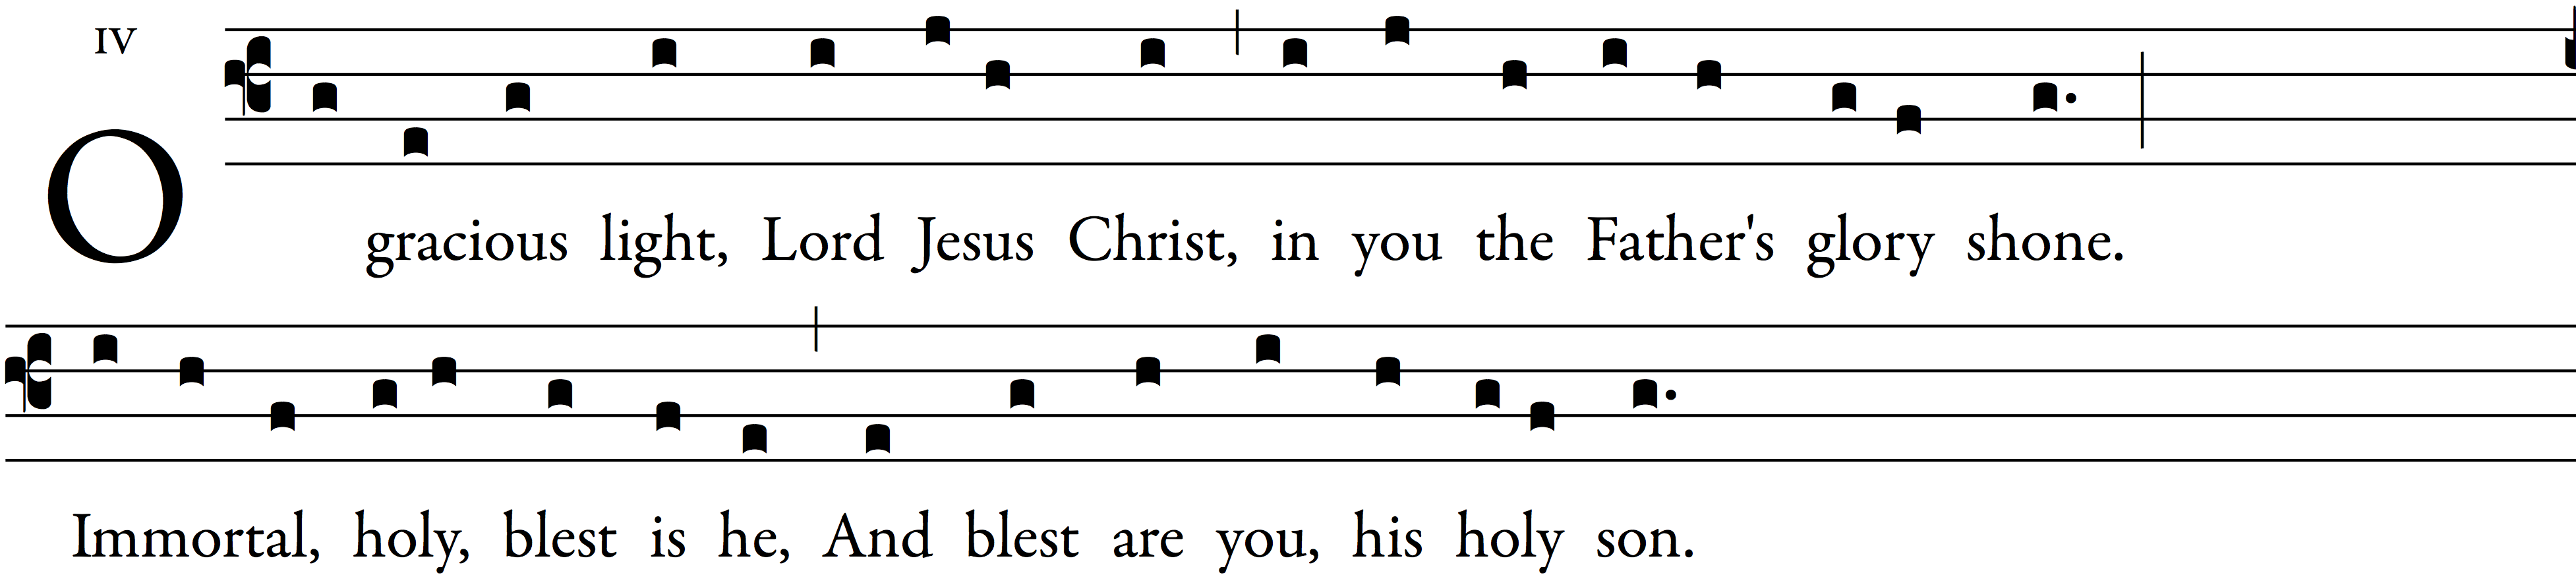
\includegraphics{phos-conditor-one.png}
\caption{}
\end{figure}

Now sunset comes, but light shines forth,\\the lamps are lit to pierce
the night.\\Praise Father, Son, and Spirit, God\\Who dwells in the
eternal light.

Worthy are you of endless praise,\\O Son of God, Life-giving
Lord;\\wherefore you are through all the earth\\and in the highest
heav'n adored.

\subsection{Psalmody}\label{psalmody}

\subsubsection{Psalm I --- \emph{Beatus vir qui non
abiit}}\label{psalm-i-beatus-vir-qui-non-abiit}

Blessed is the man that hath not walked in the counsel of the
ungodly,\\nor stood in the wáy of sínners *\\and hath not sat in the
séat of the scórnful.

2 But his delight is in the láw of the Lórd *\\and in his law will he
exercise himself dáy and night.

3 And he shall be like a tree plánted by the wáter-side *\\that will
bring forth his fruit in dúe séason.

4 His leaf also sháll not wíther *\\and look, whatsoever he doeth, ít
shall prósper.

5 As for the ungodly, it is not só with thém *\\but they are like the
chaff,\\which the wind scattereth away from the fáce of the éarth.

6 Therefore the ungodly shall not be able to stánd in the júdgement
*\\neither the sinners in the congregátion of the ríghteous.

7 But the Lord knoweth the wáy of the ríghteous *\\and the way of the
ungódly shall pérish.

Glory be to the Fáther and to the Són *\\and to the Hóly Spírit

As it was in the beginning is now and éver sháll be *\\world without
énd. Amén

\subsubsection{Psalm II --- \emph{Quare fremuerunt
gentes?}}\label{psalm-ii-quare-fremuerunt-gentes}

WHY do the heathen so furiously ràge togèther? *\\and why do the people
imàgine a vàin thing?

2 The kings of the earth stand up, and the rulers take còunsel togèther
*\\against the LORD, and agàinst his Anòinted:

3 Let us break their bònds asùnder, *\\and cast away their còrds from
ùs.

4 He that dwelleth in heaven shall làugh them to scòrn: *\\the Lord
shall hàve them in derìsion.

5 Then shall he speak unto thèm in his wràth, *\\and vex them in his
sòre displèasure:

6 Yet have I sèt my Kìng *\\upon my holy hìll of Sìon.

7 I will rehèarse the decrèe; *\\the LORD hath said unto me, Thou art my
Son,\\this day have I begòtten thèe.

8 Desire of me, and I shall give thee the nations for thìne inhèritance,
*\\and the utmost parts of the èarth for thy possèssion.

9 Thou shalt bruise them with a ròd of ìron, *\\and break them in pieces
like a pòtter's vèssel.

10 Be wise now therefore, Ò ye kìngs; *\\be instructed, ye that are
jùdges of the èarth.

11 Serve the LÒRD in fèar, *\\and rejoice unto hìm with rèverence.

12 Kiss the Son, lest he be angry,\\and so ye perish from the right
way,\\if his wrath be kindled, yèa but a lìttle. *\\Blessed are all they
that pùt their trùst in him.

\subsubsection{Psalm III --- \emph{Domine, quid
multiplicati?}}\label{psalm-iii-domine-quid-multiplicati}

LORD, how are they increased that tròuble mè! *\\many are they that rìse
agàinst me.

2 Many one there be that sày of my sòul, *\\There is no help for hìm in
his Gòd.

3 But thou, O LORD, àrt my defènder; *\\thou art my worship, and the
lìfter up of my hèad.

4 I did call upon the LÒRD with my vòice, *\\and he heard me out of his
hòly hìll.

5 I laid me down and slept, and ròse up agàin; *\\for the LÒRD sustàined
me.

6 I will not be afraid for ten thòusands of the pèople, *\\that have set
themselves agàinst me ròund about.

7 Up, LORD, and hèlp me, Ò my God, *\\for thou smitest all mine enemies
upon the cheekbone;\\thou hast broken the tèeth of the ungòdly.

8 Salvation belongeth ùnto the LÒRD; *\\and thy blessing is upòn thy
pèople.

\subsection{Lesson --- Ephesians 2:4-6
(DR)}\label{lesson-ephesians-24-6-dr}

But God, (who is rich in mercy,) for his exceeding charity wherewith he
loved us, Even when we were dead in sins, hath quickened us together in
Christ, (by whose grace you are saved,) And hath raised us up together,
and hath made us sit together in the heavenly places, through Christ
Jesus.

\subsection{Evening Canticle --- \emph{Magnificat Anima
Mea}}\label{evening-canticle-magnificat-anima-mea}

My soul doth magnify the Lord, *\\ and my spirit hath rejoiced in God my
Savior.\\For he hath regarded *\\ the lowliness of his handmaiden.\\For
behold from henceforth *\\ all generations shall call me blessed.\\For
he that is mighty hath magnified me, *\\ and holy is his Name.\\And his
mercy is on them that fear him *\\ throughout all generations.\\He hath
showed strength with his arm; *\\ he hath scattered the proud in the
imagination of their hearts.\\He hath put down the mighty from their
seat, *\\ and hath exalted the humble and meek.\\He hath filled the
hungry with good things, *\\ and the rich he hath sent empty away.\\He
remembering his mercy hath holpen his servant Israel, *\\ as he promised
to our forefathers,\\ Abraham and his seed for ever.

Glory to the Father, and to the Son, and to the Holy Spirit: * as it was
in the beginning, is now, and will be for ever.\\ Amen.

\subsection{Apostles' Creed}\label{apostles-creed}

I believe in God, the Father almighty,\\ maker of heaven and earth;

And in Jesus Christ his only Son our Lord;\\ who was conceived by the
Holy Ghost,\\ born of the Virgin Mary,\\ suffered under Pontius
Pilate,\\ was crucified, dead, and buried.\\ He descended into hell.\\
The third day he rose again from the dead.\\ He ascended into heaven,\\
and sitteth on the right hand of God the Father almighty.\\ From thence
he shall come to judge the quick and the dead.

I believe in the Holy Ghost,\\ the holy catholic Church,\\ the communion
of saints,\\ the forgiveness of sins,\\ the resurrection of the body,\\
and the life everlasting. Amen.

\subsection{The Prayers}\label{the-prayers}

\begin{description}
\itemsep1pt\parskip0pt\parsep0pt
\item[Officiant]
The Lord be with you.
\item[People]
And with thy spirit.
\item[Officiant]
Let us pray.
\end{description}

\subsubsection{The Lord's Prayer}\label{the-lords-prayer}

\begin{figure}[htbp]
\centering
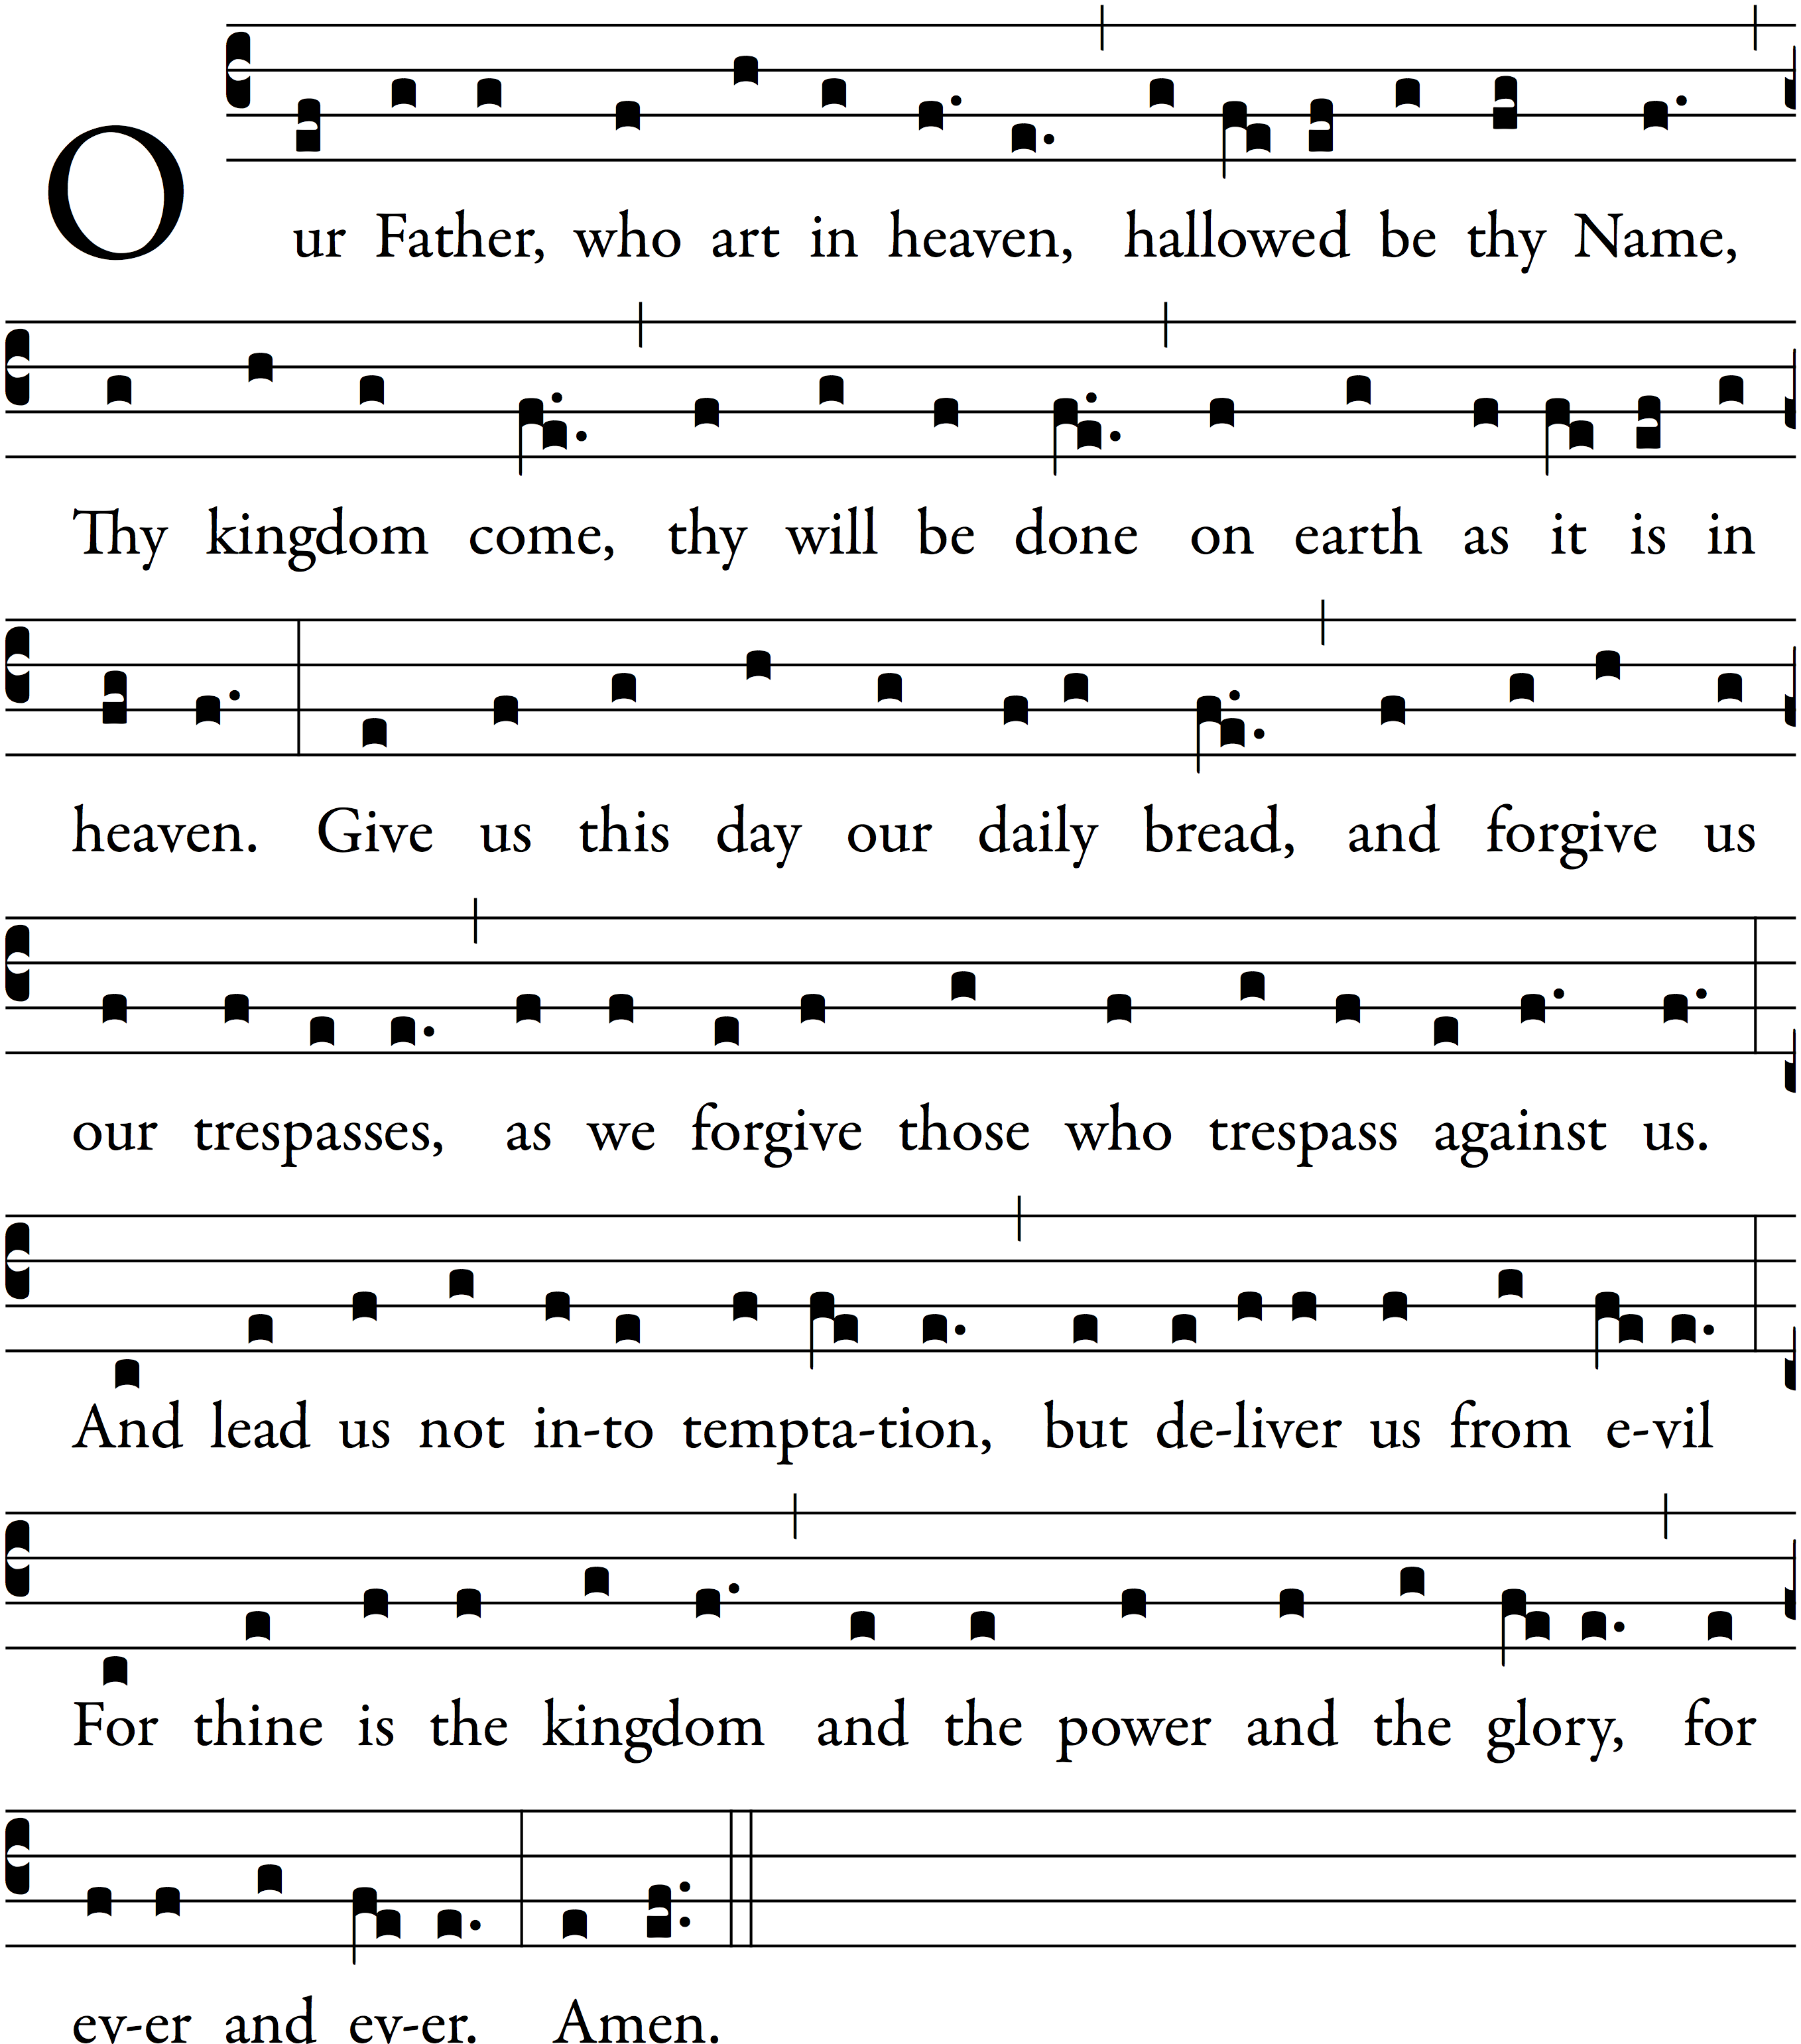
\includegraphics{lords-prayer-chant.png}
\caption{}
\end{figure}

\subsubsection{The Suffrages}\label{the-suffrages}

That this evening may be holy, good, and peaceful,\\We entreat thee, O
Lord.

That thy holy angels may lead us in paths of peace and goodwill,\\We
entreat thee, O Lord.

That we may be pardoned and forgiven for our sins and offenses,\\We
entreat thee, O Lord.

That there may be peace to thyChurch and to the whole world,\\We entreat
thee, O Lord.

That we may depart this life in thy faith and fear,\\and not be
condemned before the great judgment seat of Christ,\\We entreat thee, O
Lord.

That we may be bound together by thy Holy Spirit\\in the communion of
all thy saints,\\entrusting one another and all our life to Christ,\\We
entreat thee, O Lord.

\subsubsection{The Collects}\label{the-collects}

\paragraph{of the Day}\label{of-the-day}

Almighty God,\\ fill us with a holy joy;\\ teach us how to thank you
with reverence and love\\ on account of the ascension of Christ your
Son.\\You have raised us up with him:\\ where he, the head, has preceded
us in glory,\\ there we, the body, are called in hope.\\Through our Lord
Jesus Christ, your Son,\\ who lives and reigns with you and the Holy
Spirit,\\ one God, for ever and ever.

\paragraph{for Peace}\label{for-peace}

O God, who art the author of peace and lover of concord,\\in knowledge
of whom standeth our eternal life,\\whose service is perfect
freedom:\\Defend us, thy humble servants,\\in all assaults of our
enemies;\\that we, surely trusting in thy defense,\\may not fear the
power of any adversaries;\\through the might of Jesus Christ our Lord.

\paragraph{for this Night}\label{for-this-night}

Keep watch, dear Lord,\\with those who work, or watch, or weep this
night,\\and give thine angels charge over those who sleep.\\Tend the
sick, Lord Christ;\\give rest to the weary,\\bless the dying,\\soothe
the suffering,\\pity the afflicted,\\shield the joyous;\\and all for thy
love's sake.

\subsubsection{The General Thanksgiving}\label{the-general-thanksgiving}

Almighty God, Father of all mercies,\\we thine unworthy servants\\do
give thee most humble and hearty thanks\\for all thy goodness and
loving-kindness\\to us and to all people.

We bless thee for our creation, preservation,\\and all the blessings of
this life;\\but above all for thine inestimable love\\in the redemption
of the world by our Lord Jesus Christ;\\for the means of grace, and for
the hope of glory.

And, we beseech thee,\\give us that due sense of all thy mercies,\\that
our hearts may be unfeignedly thankful;\\and that we show forth thy
praise,\\not only with our lips, but in our lives,\\by giving up our
selves to thy service,\\and by walking before thee\\in holiness and
righteousness all our days;\\through Jesus Christ our Lord,\\to whom,
with thee and the Holy Spirit,\\be all honor and glory, world without
end.\\Amen.

\subsubsection{The Prayer of
St.~Chrysostom}\label{the-prayer-of-st.chrysostom}

Almighty God, who hast given us grace at this time, with one accord,\\to
make our common supplication unto thee;\\and hast promised through thy
well-beloved Son\\that when two or three are gathered together in his
Name thou wilt be in the midst of them:

Fulfill now, O Lord, the desires and petitions of thy servants\\as may
be best for us;\\granting us in this world knowledge of thy truth,\\and
in the world to come life everlasting.\\Amen.

\subsection{The Dismisal}\label{the-dismisal}

\begin{description}
\itemsep1pt\parskip0pt\parsep0pt
\item[Presider]
The grace of our Lord Jesus Christ, and the love of God, and the
fellowship of the Holy Ghost, be with us all evermore.
\item[All]
Amen.
\end{description}

\subsection{Seasonal Marian Hymn --- \emph{Regina
Caeli}}\label{seasonal-marian-hymn-regina-caeli}

\begin{figure}[htbp]
\centering
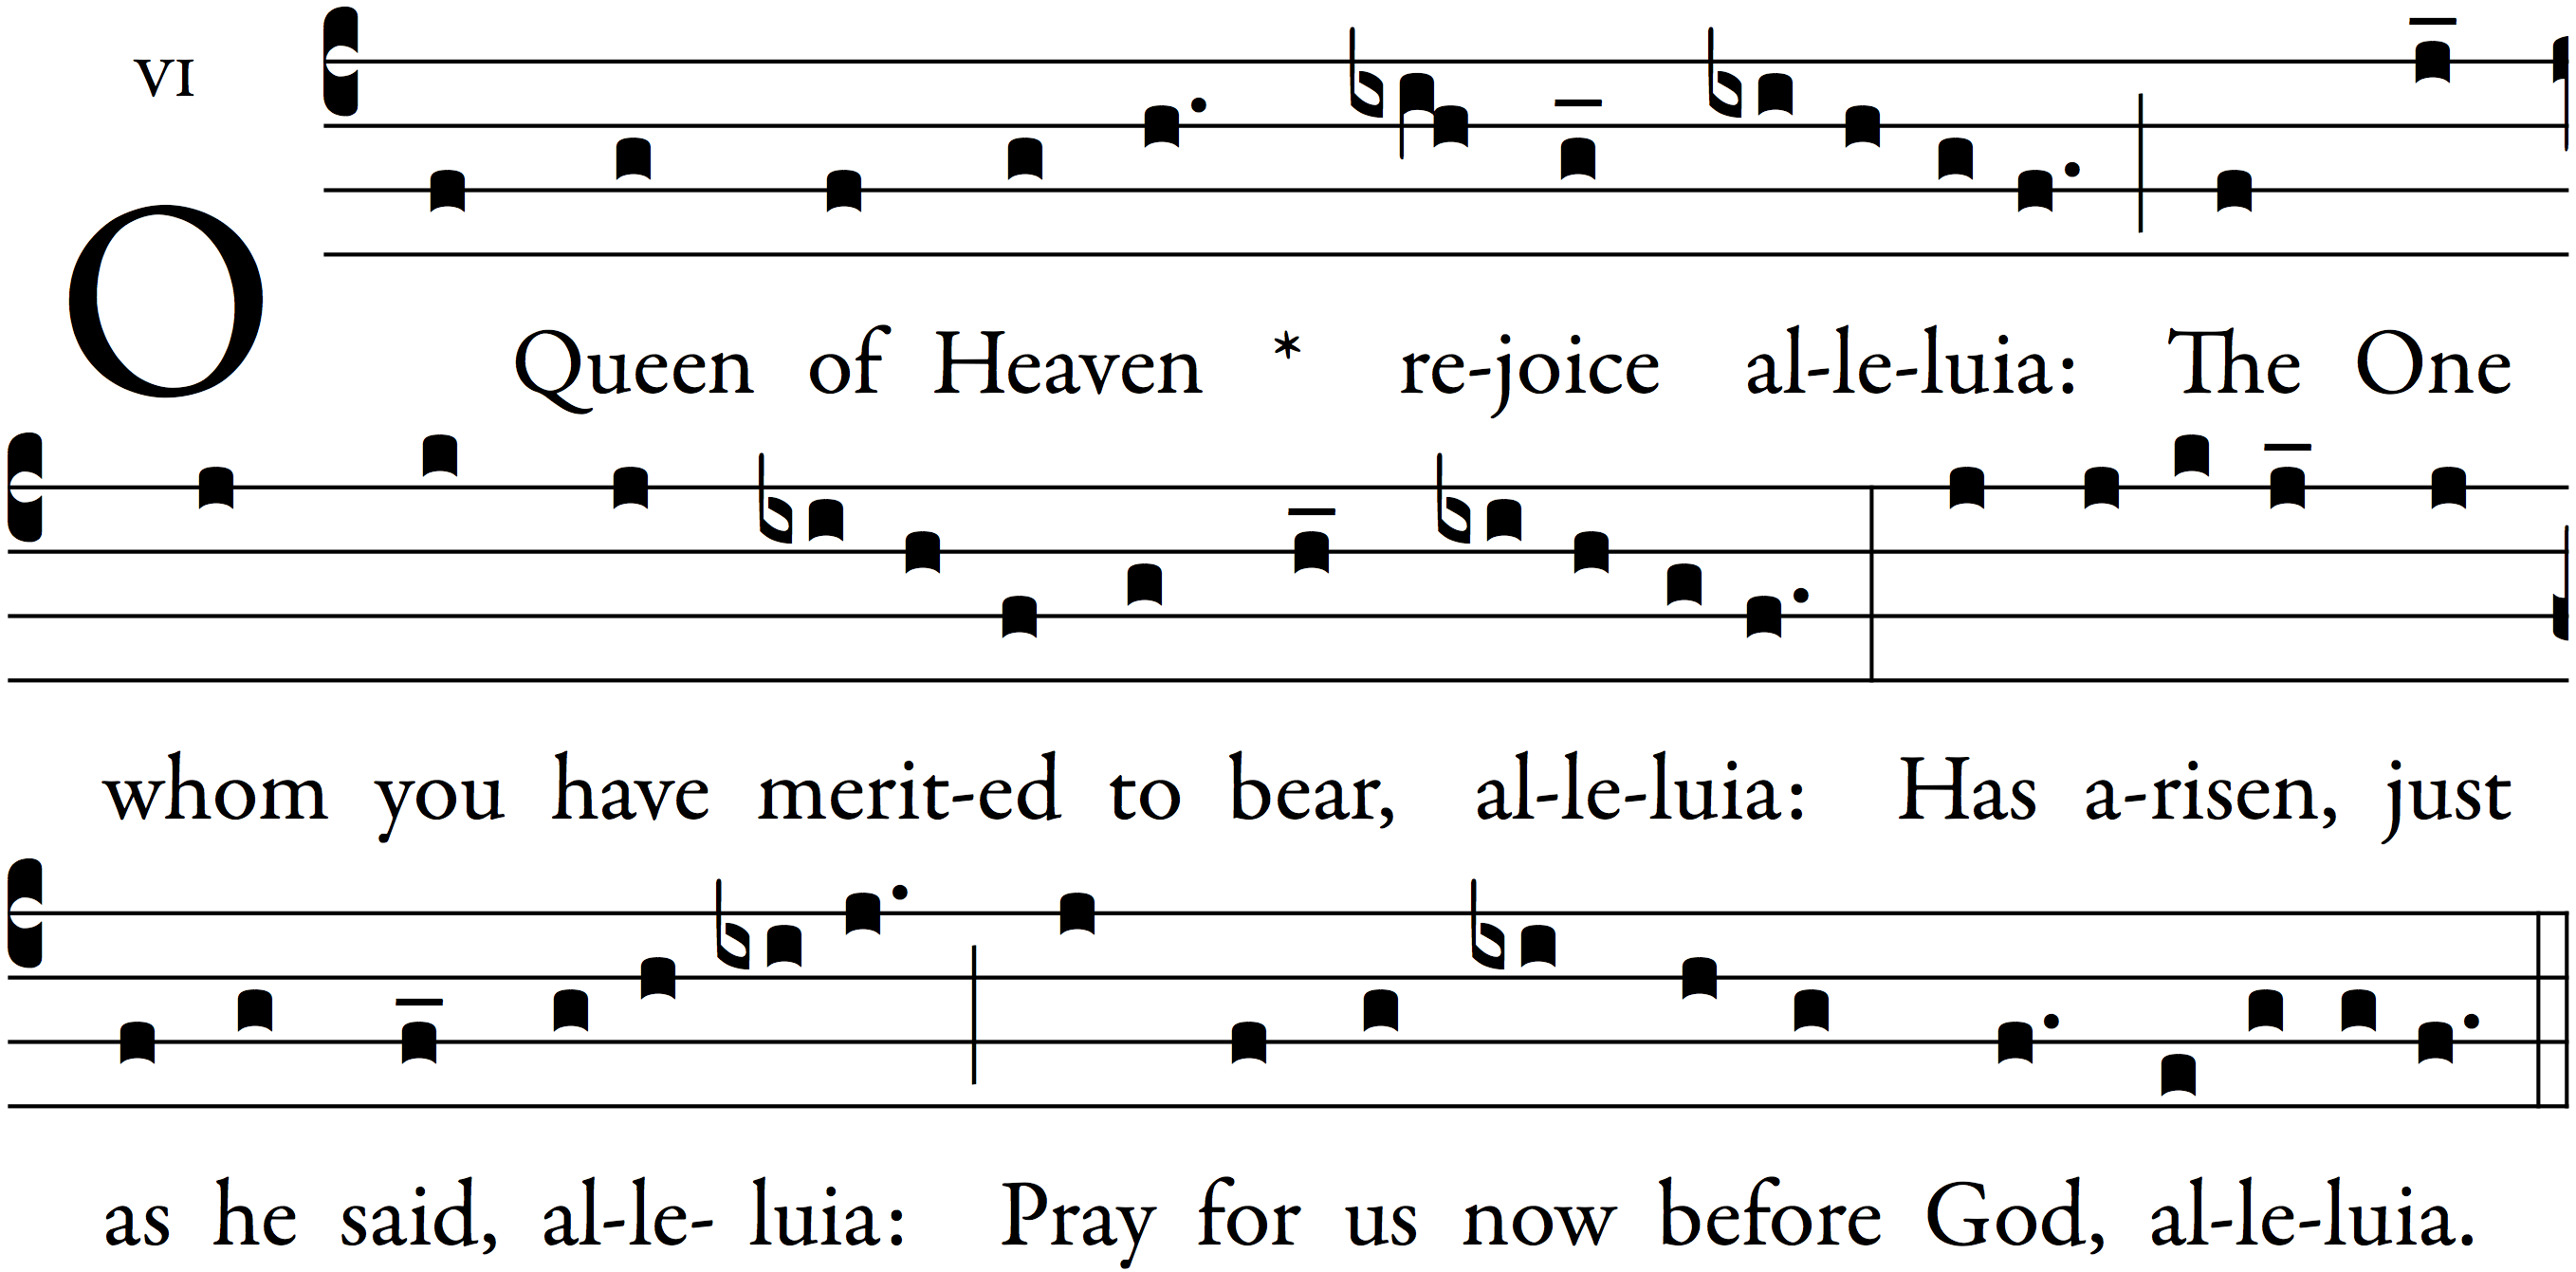
\includegraphics{regina-caeli-english.png}
\caption{}
\end{figure}

\end{document}
